\documentclass[10pt,a4paper]{article}
\usepackage[T1]{fontenc}
\usepackage{lmodern,microtype,graphicx,xcolor}
\usepackage[margin=19mm,top=16mm,bottom=17mm,footskip=8mm]{geometry}
\usepackage[colorlinks=true,urlcolor=teal!55!black]{hyperref}
\usepackage{fancyhdr}
\definecolor{ink}{HTML}{162E38}
\definecolor{accent}{HTML}{076B71}
\setlength{\parindent}{0pt}\setlength{\parskip}{5pt}\raggedbottom
\pagestyle{fancy}\fancyhf{}\renewcommand{\headrulewidth}{0pt}
\lfoot{\footnotesize\sffamily\color{accent}Stellar photometry\enspace/\enspace20 November 2026}
\rfoot{\footnotesize\sffamily\color{accent}\thepage}
\newcommand{\sub}[1]{\par\vspace{3pt}{\sffamily\bfseries\large #1}\par}
\begin{document}\color{ink}
{\sffamily\small\bfseries\color{accent}OBSERVATIONAL ASTRONOMY\hfill TESS AND BOCHUM}\par\vspace{3pt}
{\sffamily\bfseries\fontsize{23}{26}\selectfont Locating the 2.709-day eclipse near TIC 349414709\par}
A TESS eclipse published under TIC 349414705 comes from the vicinity of another star, about 15 arcseconds away. Forty TESS eclipse timings across five sectors yield a recurrence interval of \textbf{2.70917244 days}. Earlier ground-based observations recover the dimming at the same predicted phase.

\begin{center}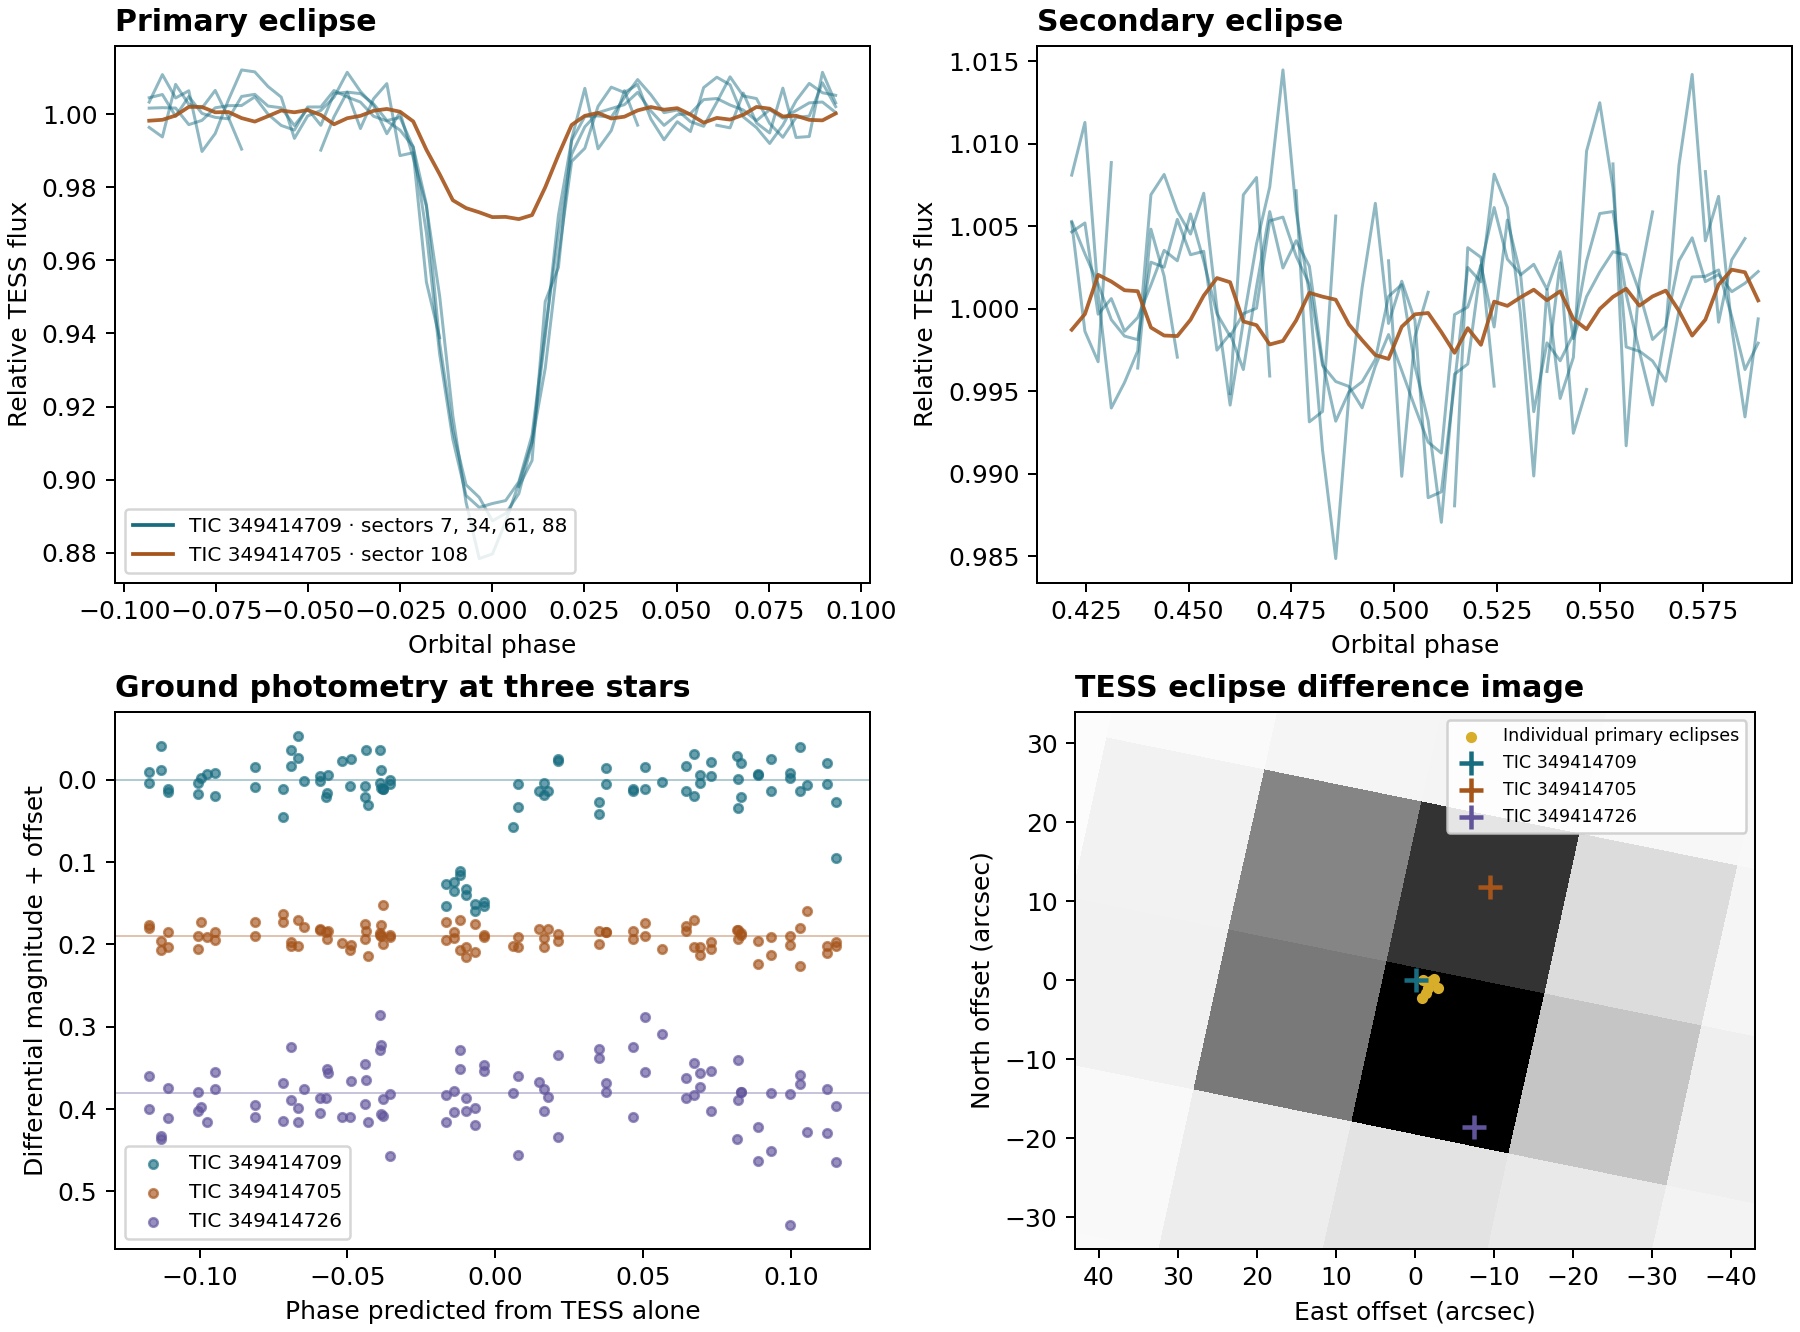
\includegraphics[width=.90\linewidth,height=99mm,keepaspectratio]{eclipse-source.png}\end{center}

\sub{Which star dims?}
In two Bochum survey bands, the source cataloged as TIC 349414709 loses \textbf{9.70\%} ($r$) and \textbf{10.67\%} ($i$) of its flux. The brighter published target changes by only 0.12\% and 0.69\% in those bands. A third star gives 0.02\% and 1.51\%. The phase windows came from TESS alone. Seven TESS eclipse difference images place the stacked center 1.93 arcseconds from TIC 349414709 at the TESS epoch. Together these tests distinguish the two catalog targets.

\sub{What was already known?}
IJspeert et al.\ (2024) listed the signal under TIC 349414705. Their reference minimum agrees with the corresponding TESS minimum here to 2.70 minutes. The nearby object measured by Bochum has Gaia DR3 identifier 5715476503089307520. Gaia resolves a second, fainter source only 0.918 arcseconds away. The available eclipse images cannot separate those two stars. This leaves the identity of the eclipsed component and its companion mass open. The likely contribution is a corrected source association and a longer-baseline ephemeris.

{\small\color{accent}\href{https://doi.org/10.1051/0004-6361/202450507}{IJspeert et al., 2024}\enspace$\cdot$\enspace\href{https://vizier.idia.ac.za/viz-bin/asu-tsv?-source=J/A\%2bA/691/A242/obaf-eb1&TIC=349414705&-out=**}{Published catalog row}\enspace$\cdot$\enspace\href{https://ui.adsabs.harvard.edu/abs/2026AN....34770087B/abstract}{Blex et al., 2026}\enspace$\cdot$\enspace\href{https://archive.stsci.edu/missions-and-data/tess}{MAST TESS archive}\enspace$\cdot$\enspace\href{https://gea.esac.esa.int/archive/}{Gaia archive}.}\par
\end{document}
